%% npj Digital Medicine Perspective template
%% Compile: latexmk -pdf main.tex
%% No strict word / reference limit; "concise" target ~2,000-2,500 body words
%% Nature referencing style (numerical superscript, sort by appearance)

\documentclass[11pt,a4paper]{article}
\usepackage[T1]{fontenc}\usepackage[utf8]{inputenc}\usepackage{lmodern}
\usepackage[margin=2.1cm]{geometry}
\usepackage{graphicx}\usepackage{amsmath,amssymb}\usepackage{booktabs}
\usepackage{caption}\usepackage{microtype}\usepackage{authblk}
\usepackage{xcolor}
\usepackage[colorlinks=true,citecolor=blue,linkcolor=blue,urlcolor=blue]{hyperref}
\usepackage[numbers,super,sort&compress]{natbib}
\usepackage{titlesec}
\titleformat{\section}{\fontsize{12}{14}\bfseries\sffamily}{\thesection}{0.6em}{}
\setlength{\parskip}{0.3\baselineskip}\setlength{\parindent}{0pt}

\title{\fontsize{15}{18}\bfseries\sffamily
The prompt is the protocol: extending the clinical-AI transparency lineage to agentic large language models}

\author[1,*]{Hsieh-Ting Lin, M.D.}
\affil[1]{Department of Hematology and Medical Oncology, Koo Foundation Sun Yat-Sen Cancer Center, Taipei, Taiwan. ORCID: 0009-0002-3974-4528.}
\affil[*]{Correspondence: \texttt{mail@hsiehting.com}.}
\date{}

\begin{document}
\maketitle\thispagestyle{empty}\vspace{-2em}

\noindent\textbf{Article type.} Perspective. \textbf{Body word count.} 1\,529 (\texttt{texcount} body sections, exclusive of abstract and declarations; npj~DM has no strict word ceiling but recommends concise writing). \textbf{References.} 11. \textbf{Figures.} 1. \textbf{Conflicts of interest.} None. \textbf{Funding.} None.

\medskip

\noindent\textbf{Abstract.} The last five years produced a sequence of clinical-AI transparency standards: Sendak's Model Facts Labels\citep{sendak2020} for deployed prediction models in 2020, the CONSORT-AI and SPIRIT-AI extensions\citep{consortAI2020} for AI-intervention trials in 2020, and TRIPOD+AI\citep{tripodAI2024} for AI-enabled prediction-model reporting in 2024. In parallel, 2026 produced two peer-reviewed Nature papers --- Co-Scientist\citep{coscientist2026} and the Sakana end-to-end AI Scientist\citep{luSakana2026} --- demonstrating that agentic large-language-model workflows can autonomously perform manuscript-grade scientific reasoning. No corresponding transparency standard exists for the agentic-LLM research class. We propose Disclosure 2.0: a six-item manifest (prompts, model identifier and tool envelope, commit history, reviewer-subagent transcripts, audit log, tagged release with a persistent DOI) that extends the Model Facts Labels and TRIPOD+AI lineage to agentic-LLM-assisted research. The present Perspective and its supporting hepatocellular-carcinoma overall-survival case study are themselves produced under Disclosure 2.0, with the case study returning a preregistered null on external validation and a sealed Layer-2 audit filing twelve substantive findings; both outcomes are visible in the public record because the disclosure regime is designed to make them visible.

\section{The clinical-AI transparency lineage}

Clinical machine learning has been on a five-year arc toward more granular transparency. In 2020 Sendak and colleagues at Duke proposed \emph{Model Facts Labels}\citep{sendak2020}: a one-page summary attached to a deployed ML model, modelled on the FDA's drug-facts label, that lists the model's intended population, performance metrics, validation history, contraindications, and human-oversight expectations. In the same year, the CONSORT-AI and SPIRIT-AI extensions formalised reporting requirements for AI-intervention randomised trials and trial protocols, respectively\citep{consortAI2020}. In 2024, TRIPOD+AI\citep{tripodAI2024} extended the long-standing TRIPOD prediction-model reporting framework to AI-enabled models with item-level guidance on training-validation-test splits, performance metric choice, calibration, fairness analysis, and code-and-data availability. Three properties characterise this lineage: \emph{atomic disclosure units} (model card, trial-report checklist, prediction-model checklist), \emph{community-endorsed schemas} (CONSORT-AI was led by SPIRIT-AI/CONSORT-AI Working Group with 40+ stakeholder organisations; TRIPOD+AI has equivalent endorsement), and \emph{venue-side adoption} (Lancet Digital Health, Nature Medicine, npj Digital Medicine and JAMA Network journals all reference these standards in their information-for-authors pages).

\section{The agentic-LLM gap}

The transparency lineage above assumes the disclosed unit is \emph{a model or a trial}. In 2026, that assumption broke. Google DeepMind's Co-Scientist\citep{coscientist2026} generated, critiqued and refined biomedical research hypotheses, with proposed acute-myeloid-leukaemia drug-repurposing candidates validated \textit{in vitro}; the Sakana AI Scientist\citep{luSakana2026} produced a manuscript that passed first-round blind workshop peer review at a top-tier machine-learning venue, the first AI-authored paper to do so. Zou and Topol\citep{zouAgentic2025} reframed agentic AI as a clinical-care teammate in The Lancet. The Nature companion editorial\citep{natureEditorial2026} called explicitly for institutions, funders and publishers to respond. None of the existing transparency standards \emph{name the artefact} that an agentic LLM produces: it is not a fixed predictive model with stable weights and an intended-use population, it is not a clinical trial, and the methods section in a 2023 sense cannot describe it because it is itself a sequence of prompt-driven LLM invocations against a moving target. In parallel, a clinician without large-lab affiliation can in 2026 assemble such a workflow on commodity tooling (Anthropic Claude via the Claude Code CLI, public TCGA and GEO data, Python and LaTeX). The present biomedical-journal AI policies, calibrated for a 2023 generation of LLM use\citep{lancetaipolicy2024}, classify almost every action such a workflow performs as prohibited and ask for a single-sentence acknowledgement in the Acknowledgements section. Prohibition without an audit surface invites camouflage rather than catching the harms current policies fear: authorship inflation, scientific hallucination (Zhao et al.\citep{zhaoHallucinations2026} document 146\,932 hallucinated citations in 2025 across arXiv, bioRxiv, SSRN and PubMed Central), and undocumented intervention.

\section{Disclosure 2.0}

We propose to extend the Model Facts Labels and TRIPOD+AI lineage with a transparency standard whose disclosed unit is the \emph{agentic-LLM-assisted research process}. The published manifest is six items at a tagged release. (1) \emph{The prompts}: every orchestration prompt committed verbatim, in order, attributed to the operator, closed for edits after first push --- the operational analogue of TRIPOD+AI's training-procedure description, but with the actual instructions rather than a paraphrase. (2) \emph{Model identifier and snapshot}: vendor, name, version, snapshot date, sampling parameters, and the tool envelope (the list of tools the model was authorised to invoke); together this is the reproducibility unit, analogous to Sendak's "intended use" and "validation history" fields. (3) \emph{The commit history}: a single repository whose git log is the chronological narrative, with force-pushes, rebases and history-rewriting forbidden. (4) \emph{The reviewer-subagent transcripts}: when reviewer subagents critique the manuscript during preparation, their outputs are committed verbatim per round, including comments later overruled, analogous to peer-review-history publication policies. (5) \emph{The audit log}: a sealed subagent produces three sub-artefacts, each compliance-relevant on its own --- (5a) re-execution from a clean clone, (5b) citation veracity against Crossref or PubMed including in-text claim-to-source alignment, and (5c) headline-statistic re-derivation. Partial discharge of (5a) alone does not satisfy item 5. (6) \emph{The tagged release with persistent DOI}: a Zenodo (or equivalent) mint bundles the manuscript PDF, LaTeX, code, transcripts, audit log, and the JSON-schema manifest validating the other five items. A \emph{minimum viable manifest} (items 1, 2, 3 and 6) preserves the consequential audit surfaces at near-zero infrastructure cost and is the recommended on-ramp for clinician-investigators without git fluency or institutional compute. A vigorous human-in-the-loop school exemplified by the Academic Research Skills toolkit\citep{ars2026} argues for AI under explicit operator supervision rather than autonomous use; the two regimes are different equilibria with different cost-of-error profiles, and Disclosure 2.0 is the \emph{orthogonal} layer underneath both: an ARS-style copilot user emits the same six-item manifest that an autonomous-pipeline user does. Figure~\ref{fig:ledger} is the artefact ledger of the supporting case study under this manifest.

\begin{figure}[h]\centering
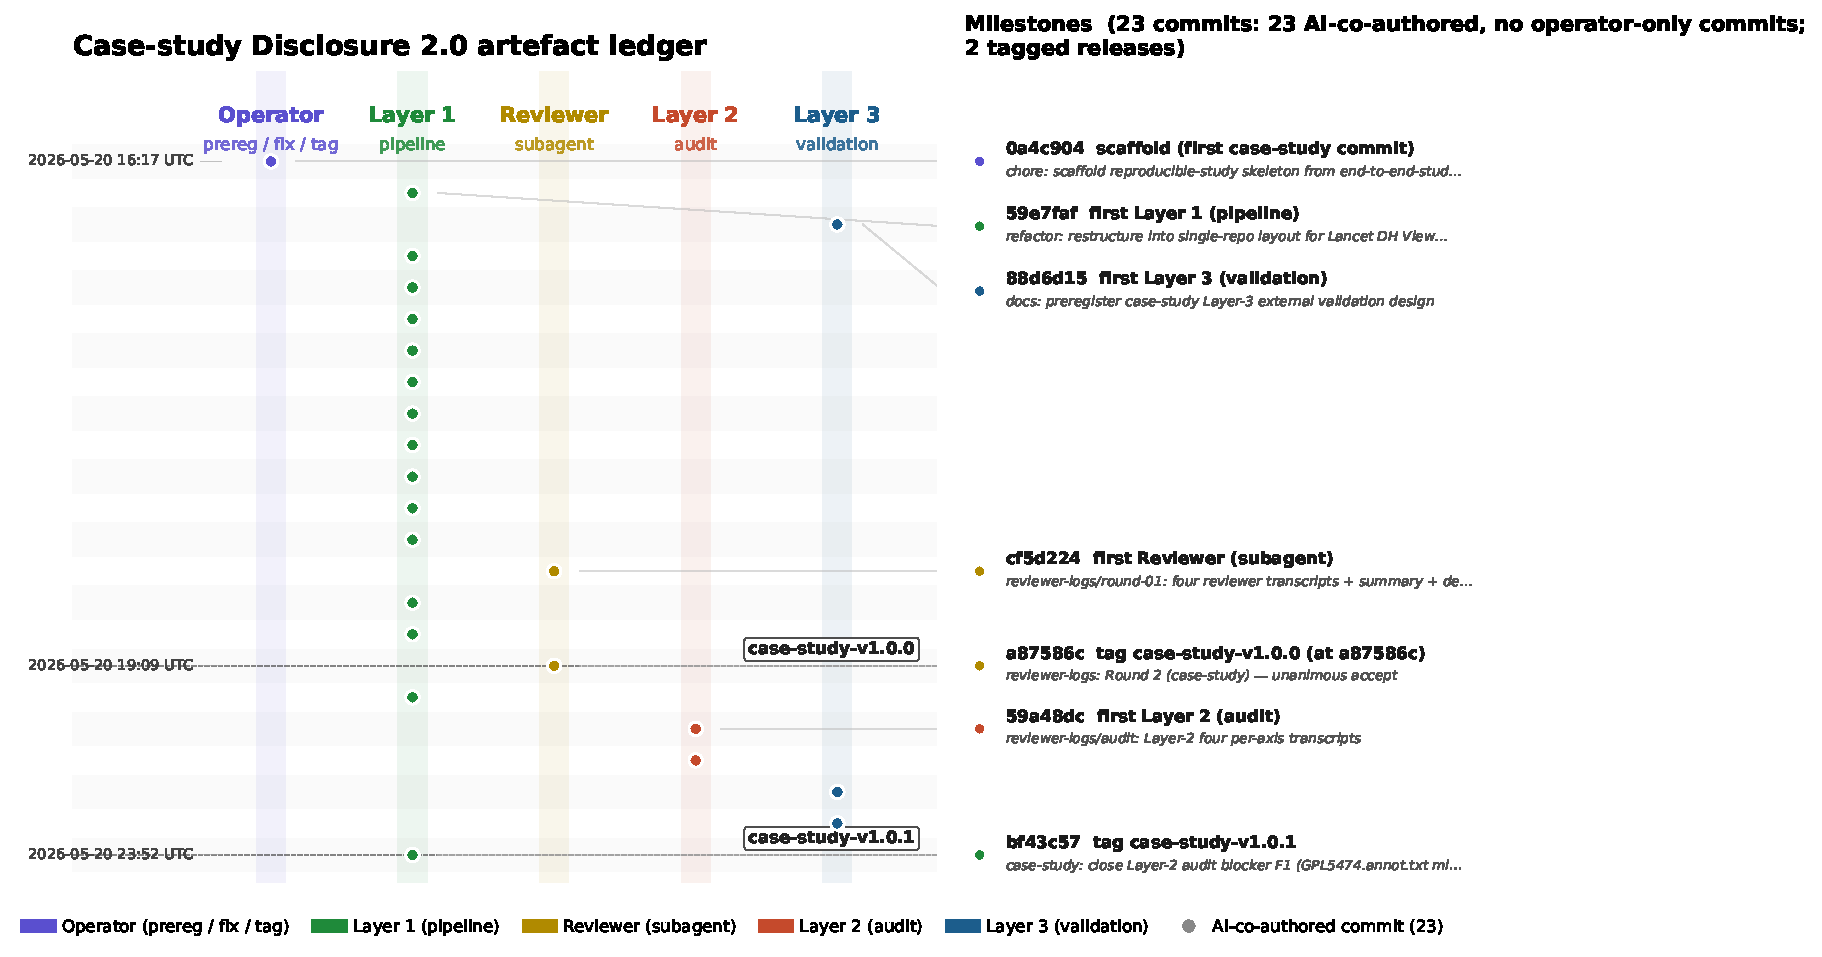
\includegraphics[width=0.92\textwidth]{figures/fig1-artifact-ledger.pdf}
\caption{Disclosure 2.0 artefact ledger for the supporting hepatocellular-carcinoma case study (the present Perspective's own commits and tags are deliberately excluded so the ledger documents the case-study disclosure unit rather than the meta-process of writing this Perspective). 23 case-study commits across five swimlanes (Operator preregistration / fixes / tags, Layer~1 pipeline, Reviewer subagents, Layer~2 audit, Layer~3 validation); two tagged releases. Marker shape encodes commit authorship (circle = AI-co-authored, square = operator-only); colour encodes swimlane. The right panel lists milestone commits (first commit per layer, tagged releases, HEAD). The ledger is regenerated from \texttt{git log} on each release tag.}\label{fig:ledger}\end{figure}

\section{The supporting case study (null on external validation)}

The supporting case study runs Disclosure 2.0 on a hepatocellular-carcinoma (HCC) overall-survival stratification problem outside the operator's clinical sub-specialty (haematology and medical oncology); TCGA-LIHC is MIT-redistributable whereas the operator's hematology raw data lives behind institutional firewalls, and the cross-domain mismatch is itself the sharper test of whether the workflow generalises. Reporting follows TRIPOD+AI for the prognostic-model component and STROBE for cohort description. Layer 1 (a single autonomous Claude Code session) produced a 50-gene transcriptomic risk score (HCC-TRS) with development-cohort paired-optimism $\Delta C$-index = 0.063, 95\,\% CI [0.003, 0.113], $n=366$ tumour samples, 130 OS events. Layer 2 (a sealed audit subagent) filed twelve substantive findings: one blocker (a required GPL annotation file not downloaded by the data-prep script, so the external-cohort branch could not be regenerated from a clean clone), two high (an abstract figure quoting the legacy estimator rather than the paired-optimism estimator the Methods specify; a stratified-vs-stage-adjusted hazard ratio discrepancy of 7.34 vs 6.66), and nine medium and low (a fabricated citation DOI to an unrelated guideline; a Jaccard-stability claim disagreeing with the saved JSON; uncited bibliography entries). None of these were caught by the within-Layer-1 reviewer rounds, which closed at unanimous accept. Layer 3 (the operator's preregistered\citep{repoprereg} external validation against held-out GSE14520 and GSE76427, pooled $n=333$, 107 events) returned $\Delta C = 0.006$, 95\,\% bootstrap CI [$-0.008$, $0.030$]; primary hypothesis \emph{not rejected}. Cohort-specific: $\Delta C = 0.016$ [$-0.010$, $0.047$] in GSE14520 ($n=219$) and $\Delta C = 0.026$ [$-0.020$, $0.141$] in GSE76427 ($n=114$). The seven preregistered secondaries (cohort-specific $\Delta C$, calibration slope at 1/3/5 years, decision-curve net benefit at thresholds 0.1/0.2/0.3, IDI at 5 years) are at \texttt{case-study/data/results/layer3\_validation.json}; calibration drifts from $\approx 1.1$ at 1\,y to $\approx 1.9$ at 5\,y, IDI~$\approx 0$, both consistent with the primary null. The development-cohort positive does not transport. The null is the headline; the manifest preserves it together with the twelve audit findings. A case study that returns null \emph{and} has twelve audit findings is the most rigorous test the disclosure standard can face. Two limits we acknowledge rather than deflect: Disclosure 2.0 does not eliminate failure modes --- it makes them findable, and findability still requires someone to look; and a single case study is not evidence the regime works at scale.

\section{Counter-arguments and rebuttals}

\emph{Prompt is not bit-deterministic.} True at the bit level, false at the level a methods section operates. Disclosure 2.0 commits to \emph{distributional reproducibility}: re-running Layer~1 at the same model identifier, snapshot date and tool envelope must yield the same selected sub-claim and statistical method across three independent runs, with the headline effect size within the original's bootstrap 95\,\% interval. \emph{A single operator cannot audit himself.} Layer 2 is a sealed audit subagent; Layer 3 is preregistered before Layer 1 sees the data; reviewer personas are diversified; the repository is open to third-party re-audit. The seal is testimonial rather than cryptographic; a session-launch attestation is the minimum operational evidence. \emph{Reviewer subagents hallucinate.} They do. The first reviewer round of the present Perspective caught three forward references to artefacts not yet committed; resolution is in the commit history, not in silent edits. \emph{This proposal is for well-resourced submitters only.} The full manifest assumes git fluency, a Zenodo account and a public tag. The minimum viable manifest preserves the consequential audit surfaces at near-zero infrastructure cost; the present repository is MIT-licensed as a forkable worked example. \emph{The audit subagent has its own hallucinations.} Cross-model audit (Layer 2 on a different vendor than Layer 1) is the proposed mitigation; the schema's \texttt{models} array supports explicit declaration.

\section{Recommendation}

npj Digital Medicine and the wider Nature-portfolio digital-health journals should pilot Disclosure 2.0 as an alternative submission track for AI-deep manuscripts. Implementation does not require Editorial Manager feature development: in a 90-day pilot, submitting authors upload a Disclosure 2.0 PDF manifest alongside the cover letter, the editorial office validates the linked Zenodo DOI against a JSON schema (a reference schema accompanies this Perspective in the linked repository at \texttt{docs/disclosure2-schema.json}), and reports on whether the manifest changes triage time, post-acceptance copy-edit burden, or reviewer-flagged hallucination rate. Five to ten npj DM submissions per quarter are a sufficient sample. The pilot's outcome metric is whether the manifest is actually \emph{consulted} by reviewers and editorial staff, not merely published: a manifest no one reads has no disciplinary effect on the failure modes it is designed to catch. A complementary recommendation: cross-model audit (Layer 1 on Anthropic Claude, Layer 2 on Google Gemini or OpenAI GPT) should be treated as the next-generation default; the schema's \texttt{models} array supports this and same-vendor audits should be treated as the single-rater-study equivalent. The Perspective the reviewer is reading was assembled under exactly that standard; every artefact the manifest would require is publicly archived at \texttt{https://github.com/htlin222/end-to-end} under MIT licence at tag \texttt{viewpoint-npjdm-v1.0.0}, with a Zenodo DOI minted on tag push. The medium is the message.

\section*{Declarations}
\noindent\textbf{Conflicts of interest.} None. \textbf{Funding.} None. \textbf{Role of the funding source.} No funder; full repository access and final submission decision rest with the author. \textbf{Generative-AI use.} Manuscript drafted with Anthropic Claude (Opus 4.7, 1M-context variant) via the Claude Code CLI; per-step disclosure log at \texttt{docs/ai-usage-disclosure.md} in the linked repository. No AI tool is listed as an author; no AI tool generated figures. \textbf{Data and code availability.} All artefacts at \texttt{https://github.com/htlin222/end-to-end} (MIT licence; tag \texttt{viewpoint-npjdm-v1.0.0}).

\bibliographystyle{vancouver}
\bibliography{references}
\end{document}
